% =====================================================================
% Project: Software Engineering (DLMCSPSE01)
% Portfolio Part 1 -- Conception Phase
% Compile: pdflatex phase1_report.tex  (run twice for the table of contents)
% Requires: logo.png in the same directory
% =====================================================================
\documentclass[a4paper,11pt]{article}

\usepackage[top=2cm, bottom=2cm, left=2cm, right=2cm]{geometry}
\usepackage[utf8]{inputenc}
\usepackage[T1]{fontenc}
\usepackage{helvet}
\renewcommand{\familydefault}{\sfdefault}
\usepackage{setspace}
\onehalfspacing
\usepackage{parskip}
\setlength{\parskip}{6pt}
\setlength{\parindent}{0pt}
\usepackage{graphicx}
\usepackage{tikz}
\usetikzlibrary{shapes.geometric, arrows.meta, positioning, calc, fit, backgrounds}
\usepackage{booktabs}
\usepackage{tabularx}
\usepackage{hyperref}
\hypersetup{colorlinks=true, linkcolor=black, citecolor=blue, urlcolor=blue}
\usepackage[round]{natbib}
\usepackage{fancyhdr}
\usepackage{caption}
\usepackage{subcaption}
% Keep the List of Figures to one entry: panels (a) and (b) belong to one figure.
\captionsetup[subfigure]{list=false}
\usepackage{enumitem}
\usepackage{xcolor}
% colortbl (not xcolor's [table] option) because TikZ already loads xcolor
\usepackage{colortbl}
\usepackage{float}
\usepackage{xurl}

\pagestyle{fancy}
\fancyhf{}
\fancyfoot[C]{\thepage}
\renewcommand{\headrulewidth}{0pt}

\usepackage{titlesec}
\titleformat{\section}{\normalfont\fontsize{12}{14}\bfseries}{\thesection}{1em}{}
\titleformat{\subsection}{\normalfont\fontsize{11}{13}\bfseries}{\thesubsection}{1em}{}
\titlespacing*{\section}{0pt}{10pt}{4pt}
\titlespacing*{\subsection}{0pt}{8pt}{3pt}

\tikzset{
  block/.style  = {draw, rounded corners=2pt, align=center, font=\scriptsize,
                   minimum height=0.8cm, inner sep=4pt},
  system/.style = {block, fill=blue!12, draw=blue!55, minimum width=3.6cm,
                   minimum height=1.2cm, font=\scriptsize\bfseries},
  actor/.style  = {draw, ellipse, fill=gray!12, align=center, font=\scriptsize, inner sep=3pt},
  ext/.style    = {block, fill=gray!12},
  layer/.style  = {block, fill=blue!8, draw=blue!45},
  comp/.style   = {block, fill=white, draw=black!45, minimum width=3.1cm},
  flow/.style   = {-{Latex[length=2mm]}, thick, draw=black!65},
  dep/.style    = {-{Latex[length=2mm]}, thick, draw=blue!60}
}

\begin{document}

% =====================================================================
% TITLE PAGE
% =====================================================================
\begin{titlepage}
\thispagestyle{empty}

\noindent

\includegraphics[width=7cm]{logo.png}

\vspace{1.2cm}
\noindent\rule{\textwidth}{0.6pt}

\vspace{0.15cm}
\begin{center}
{\Large\textbf{PortfolioCheck: Conception of a Web Application\\for the Automated Verification of Formal\\Coursework Submission Requirements}}
\end{center}
\vspace{0.05cm}
\noindent\rule{\textwidth}{0.6pt}

\vspace{1.5cm}
\begin{center}
{\large\textbf{Course: Project: Software Engineering (DLMCSPSE01)}}
\end{center}

\vspace{1.2cm}
\begin{center}
{\large\textbf{Portfolio Part 1 --- Conception Phase}}
\end{center}

\vspace{1.0cm}
\noindent
\begin{tabular}{@{}p{5.5cm} p{7cm}@{}}
\\[0.6cm]
\textbf{Degree Programme:}     & \textbf{Master of Science (M.Sc.)} \\[0.9cm]
\textbf{Name of Author:}       & \textbf{Siva Kondaru} \\[0.9cm]
\textbf{Matriculation Number:} & \textbf{10243569} \\[0.9cm]
\textbf{Name of Tutor:}        & \textbf{Holger Klus} \\[0.9cm]
\textbf{Date:}                 & \textbf{August 2026} \\[0.9cm]
\end{tabular}
\end{titlepage}

% =====================================================================
% FRONT MATTER
% =====================================================================
\pagenumbering{Roman}
\setcounter{page}{2}

\section*{Abstract}
\addcontentsline{toc}{section}{Abstract}

This document presents the conception phase of \textit{PortfolioCheck}, a
planned web application that checks a coursework portfolio submission against
the formal requirements of its assignment brief before the student hands it in.
Formal requirements --- a prescribed naming pattern, a fixed folder structure,
permitted file formats, a file-size ceiling and mandatory auxiliary artifacts
--- are mechanical and individually trivial, yet they are verified by hand under
deadline pressure and carry an explicit weight in the assessment scheme. The
report defines the project profile, selects and justifies a software development
methodology, derives the functional and non-functional requirements, establishes
the domain vocabulary, and presents the system design as a scope and context
view together with a building block view. The planned outcome of the overall
project is a browser-based, containerised application that evaluates a
submission against a set of independently testable rules and returns a report in
which every negative verdict is paired with a concrete corrective action. This
document covers planning and design only; no implementation activities or
results are reported.

\textbf{Keywords:} software engineering, requirements engineering, software
architecture, compliance checking, agile methodology

\newpage
\tableofcontents
\vspace{0.8cm}
\listoffigures
\vspace{0.4cm}
\listoftables
\newpage

% =====================================================================
% MAIN TEXT
% =====================================================================
\pagenumbering{arabic}
\setcounter{page}{1}

\section{Introduction}\label{sec:intro}

\subsection{Background}\label{subsec:background}

Every portfolio submission in a distance-learning degree programme is governed
by a set of purely formal provisions: how the archive and its main directory
must be named, which subdirectories must exist and under exactly which names,
which file formats are permitted, how large a file may be, and which auxiliary
artifacts must accompany the deliverable. These provisions exist so that
examination offices can process large volumes of submissions consistently ---
the same pressure of scale and uniformity that motivates automation elsewhere in
educational assessment \citep{Paiva2022} --- and they are stated in the
assignment brief as prose sentences spread across several chapters.

Four characteristics make these provisions a suitable target for automation.
They are deterministic, since a directory either carries the prescribed name or
it does not. They are verifiable without human judgement, since no
interpretation of the student's argument is needed to decide whether a file
exceeds a size limit. They are numerous, as a single brief may impose twenty or
more. Finally, they are checked at the worst possible moment --- in the final
hours before a deadline, when attention is directed at the content of the work
and the working memory available for mechanical detail is at its most depleted
\citep{Hermans2021}.

Automated assessment in computing education is an established field with a
mature tool landscape \citep{Paiva2022, Messer2024}. That literature is, however,
concerned almost entirely with the \textit{content} of student work: the
correctness of submitted code and the generation of feedback on solutions.
Classifications of the available techniques and tools bear this out, organising
the field around static analysis, dynamic testing and feedback generation
applied to program code \citep{Combefis2022}. The formal envelope surrounding a
submission has received very little attention,
although it is far easier to verify mechanically than program correctness and
carries a direct penalty when violated. This gap defines the opportunity
addressed by the project.

\subsection{Problem Statement and Objective}\label{subsec:problem}

Students currently verify formal requirements by re-reading the brief and
inspecting their folder structure by hand. The procedure is slow, is performed
exactly when the student is least able to perform it reliably, and offers no
confirmation of success: a student who finds no error cannot distinguish a
compliant submission from an incomplete check. Errors that survive are
discovered only after the deadline, when they can no longer be corrected --- the
familiar case of feedback arriving too late to be acted upon, which automated
tooling in education exists precisely to prevent \citep{Messer2024}.

The objective of the project is therefore to design and build a web application
that accepts the archive a student intends to submit, evaluates it against the
formal requirements, and returns an itemised report stating for each requirement
whether it is satisfied and, where it is not, precisely what must be changed.
The last element is decisive: a report that states only that something is wrong
reproduces the student's original problem in a different form, whereas feedback
that names the required correction is what gives automated assessment its
practical value \citep{Combefis2022}.

\section{Project Profile}\label{sec:profile}

\subsection{Scope and Delimitation}\label{subsec:scope}

Two commitments shape the whole design. First, the application judges
\textit{form and never content}; it makes no statement about the quality,
correctness or originality of the work and is explicitly not an assessment tool.
Second, the application \textit{does not retain submissions}; an uploaded
archive is processed and discarded within a single request. Both are carried
forward as the non-functional requirements NFR3 and NFR6 rather than as informal
intentions, so that each is attached to a defined quality characteristic and can
be verified \citep{ISO25010}.

Outside the scope are grading of content, plagiarism detection, integration with
the examination platform, user accounts and persistent history, and the rules of
other institutions. Excluding user accounts is a deliberate simplification: the
application needs no identity in order to inspect an archive, and avoiding
accounts removes an entire category of security and data-protection obligations
from a project carried out by one developer in a fixed period; the smaller the
attack surface, the fewer the weaknesses that must be defended against
\citep{OWASP2021}.

\subsection{Target Group}\label{subsec:target}

The primary target group is students in distance-learning programmes who prepare
portfolio submissions independently. Within that group the application is of
greatest value to those submitting for the first time, who have not yet
internalised the conventions, and to those working close to a deadline. The
examination office benefits indirectly from a higher proportion of correctly
structured submissions, but is not a user and is therefore not a source of
requirements --- a distinction worth drawing explicitly, since conflating
beneficiaries with users is a common route to unnecessary scope
\citep{Sommerville2020}.

\subsection{Project Organization and Plan}\label{subsec:plan}

The project is carried out by a single student who occupies every role. The
roles are nonetheless named explicitly, because the activities they represent
differ in kind and each must actually be performed \citep{Sommerville2020}: the
\textit{product owner} prioritises requirements and decides scope; the
\textit{architect} establishes the decomposition and records the technology
decisions; the \textit{developer} implements components and maintains the
repository; the \textit{tester} defines the test strategy and prepares realistic
test data. The tutor is external and provides formative feedback at the end of
each phase.

The twelve-week plan follows the three portfolio phases. Weeks 1--4 cover
analysis, requirements engineering and system design, closing with Portfolio
Part 1. Weeks 5--9 cover iterative implementation of the rule engine, the rule
set and the web interface, with the architecture documentation complemented as
decisions are taken, closing with Portfolio Part 2. Weeks 10--12 cover
containerisation, cloud deployment, installation instructions and the final
abstract, and deliberately retain schedule buffer, in keeping with the
recommendation that a plan be tailored to the situation rather than adopted
wholesale \citep{Ambler2022}.

\subsection{Risks}\label{subsec:risks}

Because a considerable proportion of software projects fails to deliver on time
or to the expected quality, risks are identified at the outset and each is paired
with a mitigation \citep{Sommerville2020}. \textit{Scope creep} through the
continual addition of new rules is countered by fixing a minimum rule set for
the first increment and treating further rules as a prioritised backlog.
\textit{Ambiguity in the brief} is countered by recording the source provision
for every rule and raising open interpretations in the tutorial feedback loop.
\textit{Malicious uploads} are countered by treating every archive as hostile
input and enforcing limits before extraction, as specified in NFR1 and NFR2.
\textit{Late deployment failure}
is countered by containerising from the start and deploying a trivial increment
early. \textit{Capacity loss} in a single-developer project is countered by the
buffer in weeks 10--12 and by keeping every increment independently deliverable
--- an application of the principle that software must be built to survive
change over time rather than merely to work once \citep{Winters2020}.

One risk is specific to this class of application: a checker that misses a
violation is worse than no checker, because it converts justified uncertainty
into unjustified confidence. The mitigation is twofold --- the interface states
plainly which requirements are covered, and no rule counts as complete until an
automated test demonstrates that it rejects a submission violating it --- the
test, rather than the author's confidence, being what establishes that the rule
actually works \citep{Khorikov2020}.

\section{Software Development Methodology}\label{sec:methodology}

The project follows an \textbf{incremental, Kanban-based agile approach with
two-week timeboxes}. Work items are held in a single prioritised backlog and
visualised on a board with the states \textit{backlog}, \textit{in progress},
\textit{in review} and \textit{done}, with the work-in-progress limit set to
one. Each timebox closes with a review of the increment against the requirements
it was meant to satisfy, which keeps the flow of work visible and the amount in
progress bounded \citep{Ambler2022}.

Three considerations drove this choice over the alternatives. A
\textit{waterfall} approach would defer all working software to the end, leaving
no opportunity to act on tutorial feedback and concentrating risk at the point
where it can least be absorbed. \textit{Scrum} in its full form presupposes a
development team; its events and accountabilities cannot be meaningfully enacted
by one person \citep{Schwaber2020}. A Kanban-based flow scales down to a single
developer without ceremony while retaining the practices that generate the
benefit --- a prioritised backlog, limited work in progress, a demonstrable
increment and an explicit review \citep{Ambler2022}. The fit is reinforced by
the shape of the problem itself: each formal rule is independent of the others,
so the system can deliver value with a small rule set and grow one rule at a
time.

Four supporting practices are treated as non-negotiable. Version control uses a
public repository with small, atomic commits and annotated tags marking the
state submitted at each milestone, so that release control is demonstrable from
the repository history. Architecture documentation is versioned alongside the
source code so that the two cannot diverge silently \citep{Bass2021}. Automated
tests are written for every rule as part of the increment that introduces it
\citep{Khorikov2020}. Any requirement that cannot be met within the project
scope is recorded explicitly as technical debt rather than left unstated.

\section{Requirements}\label{sec:requirements}

The requirements are derived directly from the assignment brief, which functions
as the authoritative specification of the domain: each formal provision
translates into one verifiable rule. This gives the project an unusual advantage,
since the requirements source is written and stable, but it also imposes an
obligation --- a rule that misreads its source produces confidently wrong advice.
Every rule therefore records the provision it derives from, and that provenance
is shown to the user so the rule can be checked against the original document,
maintaining the traceability from requirement to source that requirements
engineering demands \citep{Sommerville2020}.

Non-functional requirements are organised along the product quality
characteristics of ISO/IEC 25010 \citep{ISO25010}, which supplies an established
vocabulary and keeps the list from collapsing into an unstructured set of
aspirations.

The complete requirements base is presented in Table~\ref{tab:requirements}. Its
upper block lists the twelve functional requirements FR1--FR12 with a priority
assigned according to the MoSCoW scheme; its lower block lists the nine
non-functional requirements NFR1--NFR9, each labelled with the ISO/IEC 25010
quality characteristic it belongs to \citep{ISO25010} and with the means by
which it is intended to be verified. The two blocks are separated by a double
rule so that the change of column meaning --- from priority to verification
method --- is visible at a glance.

\begin{table}[H]
\centering
\caption{Functional and non-functional requirements}
\label{tab:requirements}
\footnotesize
\renewcommand{\arraystretch}{1.25}
\setlength{\tabcolsep}{4pt}
\begin{tabularx}{\textwidth}{|c|X|p{2.9cm}|}
\hline
\rowcolor{gray!15}
\textbf{ID} & \textbf{Requirement} & \textbf{Priority / Verification} \\
\hline
\hline
\multicolumn{3}{|l|}{\cellcolor{blue!8}\textit{\textbf{Functional requirements}}} \\
\hline
FR1 & The system shall accept a submission archive uploaded through a web browser. & Must \\
\hline
FR2 & The system shall verify the name of the main directory against the prescribed pattern. & Must \\
\hline
FR3 & The system shall verify the presence and exact naming of all prescribed subdirectories. & Must \\
\hline
FR4 & The system shall verify that files declared as PDF are genuinely PDF documents, by inspecting content rather than the file extension. & Must \\
\hline
FR5 & The system shall verify that no file exceeds the prescribed size limit. & Must \\
\hline
FR6 & The system shall verify the presence and content of the auxiliary artifacts required for the applicable phase. & Must \\
\hline
FR7 & The system shall return a report giving each rule a verdict of \textit{passed}, \textit{to review} or \textit{must fix}. & Must \\
\hline
FR8 & The system shall accompany every non-passing verdict with a concrete corrective action. & Must \\
\hline
FR9 & The system shall allow the user to declare the portfolio phase and evaluate only the rules applicable to it. & Should \\
\hline
FR10 & The system shall provide a downloadable, correctly structured but empty folder skeleton. & Should \\
\hline
FR11 & The system shall display the provision of the brief from which each rule derives. & Should \\
\hline
FR12 & The system shall compare the file inventory of the submitted code archive with that of the referenced public repository. & Could \\
\hline
\hline
\multicolumn{3}{|l|}{\cellcolor{blue!8}\textit{\textbf{Non-functional requirements (ISO/IEC 25010 characteristics)}}} \\
\hline
NFR1 & \textit{Security.} The system shall reject archives containing absolute paths or relative path traversal before extraction. & Automated test, crafted archive \\
\hline
NFR2 & \textit{Security.} The system shall reject archives whose expanded size, entry count or compression ratio exceeds defined limits. & Automated test, crafted archive \\
\hline
NFR3 & \textit{Security.} The system shall delete every uploaded and extracted file before the response is returned, and persist no submission data. & Code review \\
\hline
NFR4 & \textit{Security.} The application shall run without administrative privileges on a read-only container filesystem. & Configuration review \\
\hline
NFR5 & \textit{Performance.} The system shall return a report within three seconds for a submission of typical size. & Timing during review \\
\hline
NFR6 & \textit{Usability.} The report shall be comprehensible without reference to the assignment brief. & Review against FR8 \\
\hline
NFR7 & \textit{Maintainability.} Adding a further rule shall require changes only to the rule component and its test. & Architecture review \\
\hline
NFR8 & \textit{Reliability.} A failure in one rule shall not prevent the remaining rules from being evaluated. & Automated test \\
\hline
NFR9 & \textit{Portability.} The system shall be deployable through a single container composition command. & Deployment from clean host \\
\hline
\end{tabularx}
\end{table}

Two entries deserve further comment. Requirement FR12 is the principal source of
novelty. The brief requires the
contents of the public repository and of the submitted archive to be identical
--- a provision that is effectively impossible to verify by hand and that no
existing tool addresses. It is prioritised as \textit{could} because it
introduces a dependency on an external service and must not endanger the core
increment. The security requirements are stated first among the non-functional
ones because uploading an arbitrary archive is the only genuinely hostile
interaction in the system: archive extraction is a documented source of
vulnerabilities, since a crafted entry can be written outside the intended
directory and a small archive can be built to expand until it exhausts the
host's resources. Treating all externally supplied input as untrusted, and
validating it before it reaches the component that acts on it, is the
established mitigation for this class of weakness \citep{OWASP2021}.

Verification is planned during conception rather than after implementation, which
is why a means of verification is fixed for every non-functional requirement
before any code exists. Each rule will be exercised
against a compliant submission and against one violating exactly that rule;
crafted archives will confirm each extraction limit demanded by NFR1 and NFR2;
the complete upload-to-report path will be tested through the HTTP interface;
and the container composition will be started from a clean environment to
confirm NFR9. Test data will consist of realistic submission archives rather
than placeholder content, since a test is only as convincing as the
representativeness of the data it runs against \citep{Khorikov2020}.

\section{Glossary}\label{sec:glossary}

The glossary fixes the domain vocabulary so that a term carries the same meaning
for the developer, the tutor and any future reader \citep{Sommerville2020}.

\begin{description}[leftmargin=3.4cm, style=nextline, font=\normalfont\bfseries, itemsep=1pt]
\item[Submission] The complete set of files a student intends to hand in for one
portfolio phase, supplied to the system as a single archive.
\item[Main directory] The single top-level folder inside the archive, whose name
must follow the prescribed pattern.
\item[Rule] An independently verifiable formal requirement derived from one
provision of the assignment brief.
\item[Finding] The verdict produced by evaluating one rule against one
submission: a severity, an explanatory message and, where applicable, a
corrective action.
\item[Severity] The classification of a finding as \textit{passed}, \textit{to
review} or \textit{must fix}.
\item[Report] The aggregate of all findings for one submission, with the overall
verdict derived from the most severe finding.
\item[Rule engine] The component that selects the applicable rules, evaluates
them and aggregates the resulting findings.
\item[Technical debt] A requirement consciously left unsatisfied within the
project scope, recorded together with its consequence.
\end{description}

\section{System Design}\label{sec:design}

The system design is presented in Figure~\ref{fig:design}, which combines the two
views required at this stage. Presenting an architecture as a small set of
nested views --- the system in its environment first, its internal structure
second --- is a widely adopted convention, since each view answers a different
question and remains legible on its own \citep{Brown2024}. Panel~(a) delimits
the system from its environment:
the student is the sole human user and interacts only through a web browser, the
assignment brief is not a runtime interface but the authoritative source from
which the rule set is derived, and the repository hosting service is an optional
interface needed only by FR12 and is therefore drawn with a dashed outline.
Panel~(b) decomposes the system into its building blocks and records the
dependencies between them; in the customary analogy it corresponds to the floor
plan of a building \citep{Bass2021}.

\begin{figure}[H]
\centering
\begin{subfigure}{\textwidth}
\centering
% All positions are explicit, so the layout cannot depend on declaration order.
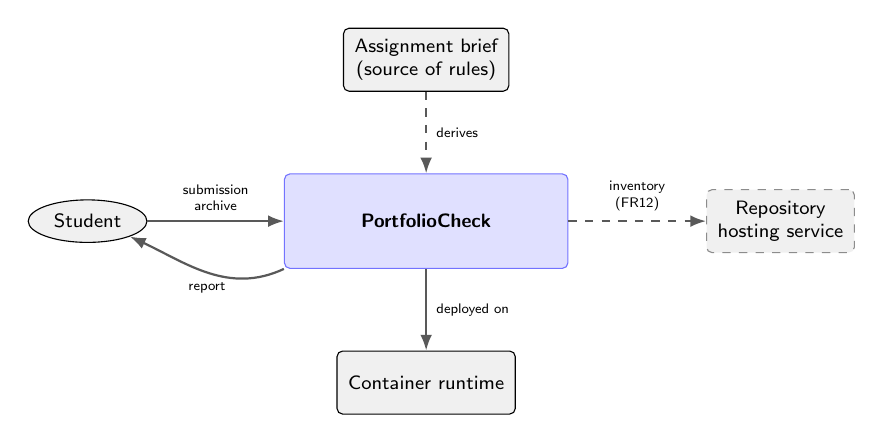
\begin{tikzpicture}
\node[system]                  at ( 0   , 0    ) (sys)     {PortfolioCheck};
\node[actor]                   at (-4.3 , 0    ) (student) {Student};
\node[ext]                     at ( 0   , 2.05 ) (brief)   {Assignment brief\\(source of rules)};
\node[ext, draw=black!45, dashed] at ( 4.5, 0  ) (vcs)     {Repository\\hosting service};
\node[ext]                     at ( 0   ,-2.05 ) (host)    {Container runtime};

\draw[flow] (student.east) -- node[above, font=\tiny, align=center]
      {submission\\archive} (sys.west);
\draw[flow] (sys.south west) to[out=205, in=335]
      node[below, font=\tiny] {report} (student.south east);
\draw[flow, dashed] (brief.south) -- node[right, font=\tiny] {derives} (sys.north);
\draw[flow, dashed] (sys.east) -- node[above, font=\tiny, align=center]
      {inventory\\(FR12)} (vcs.west);
\draw[flow] (sys.south) -- node[right, font=\tiny] {deployed on} (host.north);
\end{tikzpicture}
\caption{Scope and context}
\label{fig:context}
\end{subfigure}

\vspace{0.7cm}

\begin{subfigure}{\textwidth}
\centering
% Layer bands are drawn first so the component boxes always sit on top of them.
% Column centres: 1.55 / 5.15 / 8.75 -- band spans x = -0.30 .. 10.60
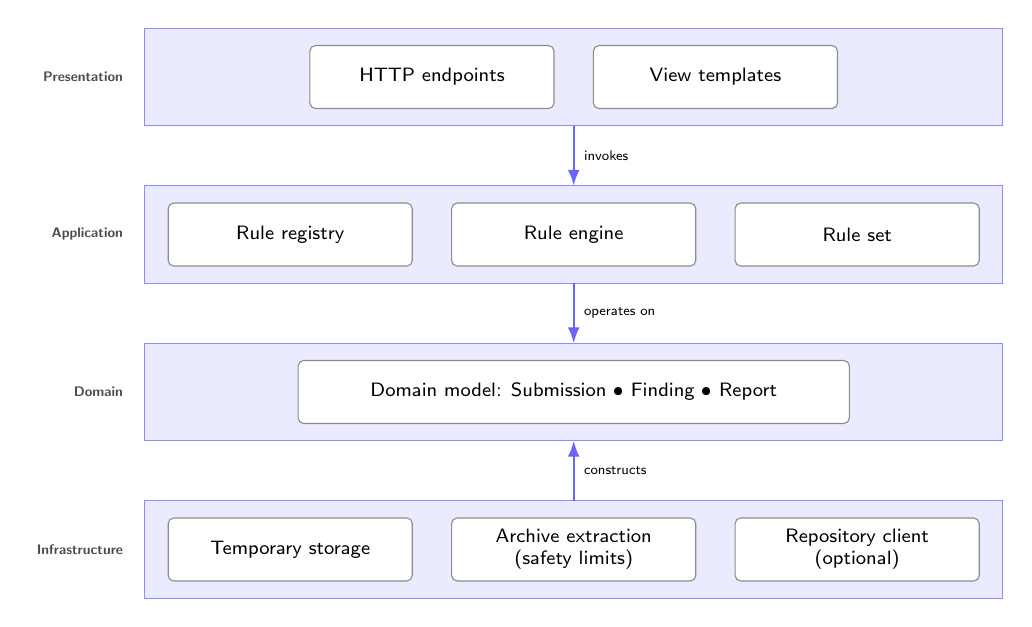
\begin{tikzpicture}[font=\scriptsize]
\foreach \y/\name in {0/Presentation, -2/Application, -4/Domain, -6/Infrastructure} {
  \fill[blue!8]  (-0.30,\y-0.62) rectangle (10.60,\y+0.62);
  \draw[blue!45] (-0.30,\y-0.62) rectangle (10.60,\y+0.62);
  \node[font=\tiny\bfseries, anchor=east, black!70] at (-0.45,\y) {\name};
}

% Presentation layer (two components, centred on the band)
\node[comp] at (3.35, 0) (routes)    {HTTP endpoints};
\node[comp] at (6.95, 0) (templates) {View templates};

% Application layer
\node[comp] at (1.55,-2) (registry) {Rule registry};
\node[comp] at (5.15,-2) (engine)   {Rule engine};
\node[comp] at (8.75,-2) (rules)    {Rule set};

% Domain layer
\node[comp, minimum width=7cm] at (5.15,-4) (model)
  {Domain model: Submission \textbullet\ Finding \textbullet\ Report};

% Infrastructure layer
\node[comp] at (1.55,-6) (tempstore) {Temporary storage};
\node[comp] at (5.15,-6) (extract)   {Archive extraction\\(safety limits)};
\node[comp] at (8.75,-6) (vcsclient) {Repository client\\(optional)};

% Dependencies, drawn vertically on the band centre line
\draw[dep] (5.15,-0.62) -- node[right, font=\tiny] {invokes}     (5.15,-1.38);
\draw[dep] (5.15,-2.62) -- node[right, font=\tiny] {operates on} (5.15,-3.38);
\draw[dep] (5.15,-5.38) -- node[right, font=\tiny] {constructs}  (5.15,-4.62);
\end{tikzpicture}
\caption{Building block view with layer dependencies}
\label{fig:blocks}
\end{subfigure}
\caption{System design: scope and context view and building block view}
\label{fig:design}
\end{figure}

This decomposition is driven directly by NFR7. Dependencies point strictly
inward, as the arrows indicate, so the domain model at the centre depends on
nothing and the outer layers depend on it \citep{Percival2020, Richards2020}. The rule set sits behind
a registry, so introducing a further formal requirement affects one component
and its test and nothing else: the presentation layer discovers the available
rules through the registry rather than knowing them individually. Keeping the
domain model free of any dependency on the web framework allows every rule to be
tested against an in-memory submission without starting a server. Archive
extraction is confined to the infrastructure layer because it is the component
that touches untrusted input, which makes the defences of NFR1 and NFR2
auditable in one location rather than dispersed across the system.

The significant technology decisions follow from these requirements. Python is
selected as the implementation language for its mature standard-library support
for archive and document handling, which is the core of the problem domain. An
ASGI-based web framework with integrated request validation \citep{FastAPI2025}
provides upload handling without additional components. The user interface is
rendered on the server, which avoids a separate front-end build pipeline and a
second deployment artifact for what is essentially a form and a report
\citep{Richards2020}. No database is used, because no requirement calls for
retaining submissions and omitting persistence removes both a component and a
data-protection obligation; should a future requirement demand it, the layered
decomposition confines the change to the infrastructure layer. Packaging uses a
container composition \citep{Docker2024}, which is required by the brief and
also guarantees that the environment described in the documentation is the
environment that runs.

\section{Conclusion and Outlook}\label{sec:conclusion}

This document has established the conception of \textit{PortfolioCheck}. The
project addresses a narrow, well-defined and largely unaddressed problem: formal
submission requirements are mechanical and carry marks, yet are verified by hand
at the least favourable moment. The profile fixes the objective, target group
and delimitation; an incremental, Kanban-based approach was selected and
justified against the conditions of a single-developer project structured by
external milestones; the requirements were derived from an authoritative written
source and organised along an established quality model; and the design was
presented as a context view and a layered building block view whose principal
driver is the ability to add a rule without disturbing the rest of the system
--- the architecture being documented in the views that make its structure
communicable rather than in prose alone \citep{Bass2021}.

The development phase will implement the components identified above, beginning
with the domain model and the rule engine, followed by the initial rule set and
the web interface, with the repository comparison of FR12 scheduled last so that
it cannot endanger the core increment. The architecture documentation will be
complemented as decisions are taken and maintained under version control
alongside the source code, on the understanding that architectural choices are
trade-offs whose consequences emerge over the life of the system rather than
settled facts established once at the outset \citep{Ford2021}.

\newpage

% =====================================================================
% REFERENCES
% =====================================================================
\section*{References}
\addcontentsline{toc}{section}{References}

\begin{thebibliography}{99}
\setlength{\itemsep}{5pt}

\bibitem[Ambler and Lines(2022)]{Ambler2022}
Ambler, S. W. and Lines, M. (2022) \textit{Choose Your WoW! A Disciplined Agile
Approach to Optimizing Your Way of Working}. 2nd edn. Newtown Square, PA:
Project Management Institute.

\bibitem[Bass et~al.(2021)]{Bass2021}
Bass, L., Clements, P. and Kazman, R. (2021) \textit{Software Architecture in
Practice}. 4th edn. Boston, MA: Addison-Wesley.

\bibitem[Brown(2024)]{Brown2024}
Brown, S. (2024) \textit{The C4 Model for Visualising Software Architecture}.
Available at: \url{https://c4model.com/} (Accessed: 8 August 2026).

\bibitem[Comb\'{e}fis(2022)]{Combefis2022}
Comb\'{e}fis, S. (2022) `Automated code assessment for education: review,
classification and perspectives on techniques and tools', \textit{Software},
1(1), pp. 3--30.

\bibitem[Docker(2024)]{Docker2024}
Docker Inc. (2024) \textit{Compose Specification}. Available at:
\url{https://docs.docker.com/compose/} (Accessed: 8 August 2026).

\bibitem[Ford et~al.(2021)]{Ford2021}
Ford, N., Richards, M., Sadalage, P. and Dehghani, Z. (2021) \textit{Software
Architecture: The Hard Parts --- Modern Trade-Off Analyses for Distributed
Architectures}. Sebastopol, CA: O'Reilly Media.

\bibitem[Hermans(2021)]{Hermans2021}
Hermans, F. (2021) \textit{The Programmer's Brain: What Every Programmer Needs
to Know about Cognition}. Shelter Island, NY: Manning.

\bibitem[ISO/IEC(2023)]{ISO25010}
International Organization for Standardization (2023) \textit{ISO/IEC
25010:2023 Systems and Software Engineering --- Systems and Software Quality
Requirements and Evaluation (SQuaRE) --- Product Quality Model}. Geneva: ISO.

\bibitem[Khorikov(2020)]{Khorikov2020}
Khorikov, V. (2020) \textit{Unit Testing Principles, Practices, and Patterns}.
Shelter Island, NY: Manning.

\bibitem[Messer et~al.(2024)]{Messer2024}
Messer, M., Brown, N. C. C., K\"{o}lling, M. and Shi, M. (2024) `Automated
grading and feedback tools for programming education: a systematic review',
\textit{ACM Transactions on Computing Education}, 24(1), pp. 1--43.

\bibitem[OWASP(2021)]{OWASP2021}
Open Worldwide Application Security Project (2021) \textit{OWASP Top 10:2021}.
Available at: \url{https://owasp.org/Top10/} (Accessed: 8 August 2026).

\bibitem[Paiva et~al.(2022)]{Paiva2022}
Paiva, J. C., Leal, J. P. and Figueira, \'{A}. (2022) `Automated assessment in
computer science education: a state-of-the-art review', \textit{ACM
Transactions on Computing Education}, 22(3), pp. 1--40.

\bibitem[Percival and Gregory(2020)]{Percival2020}
Percival, H. and Gregory, B. (2020) \textit{Architecture Patterns with Python}.
Sebastopol, CA: O'Reilly Media.

\bibitem[Ram\'{i}rez(2025)]{FastAPI2025}
Ram\'{i}rez, S. (2025) \textit{FastAPI Documentation}. Available at:
\url{https://fastapi.tiangolo.com/} (Accessed: 8 August 2026).

\bibitem[Richards and Ford(2020)]{Richards2020}
Richards, M. and Ford, N. (2020) \textit{Fundamentals of Software Architecture:
An Engineering Approach}. Sebastopol, CA: O'Reilly Media.

\bibitem[Schwaber and Sutherland(2020)]{Schwaber2020}
Schwaber, K. and Sutherland, J. (2020) \textit{The Scrum Guide: The Definitive
Guide to Scrum}. Available at: \url{https://scrumguides.org/} (Accessed:
8 August 2026).

\bibitem[Sommerville(2020)]{Sommerville2020}
Sommerville, I. (2020) \textit{Engineering Software Products: An Introduction
to Modern Software Engineering}. Harlow: Pearson Education.

\bibitem[Winters et~al.(2020)]{Winters2020}
Winters, T., Manshreck, T. and Wright, H. (2020) \textit{Software Engineering
at Google: Lessons Learned from Programming over Time}. Sebastopol, CA:
O'Reilly Media.

\end{thebibliography}

\end{document}
